% diagrams-Bd.tex
\begin{hcarentry}[updated]{diagrams}
\report{Jeffrey Rosenbluth}%11/14
\status{active development}
\participants{Daniel Bergey, Jan Bracker, Christopher Chalmers, Daniil Frumin,  Allan Gardner, Andy Gill, 
  Niklas Haas, John Lato, Chris Mears, Jeff Rosenbluth, Michael Sloan, Ryan Yates}

\makeheader

The diagrams framework provides an embedded domain-specific language
for declarative drawing.  The overall vision is for diagrams to become
a viable alternative to DSLs like MetaPost or Asymptote, but with the
advantages of being \emph{declarative}---describing what to draw, not
how to draw it---and \emph{embedded}---putting the entire power of
Haskell (and Hackage) at the service of diagram creation.  There is
still much more to be done, but diagrams is already quite
fully-featured, with a comprehensive user manual, a large collection
of primitive shapes and attributes, many different modes of
composition, paths, cubic splines, images, text, arbitrary monoidal
annotations, named subdiagrams, and more.

%**<img width=400 src="./paradox.jpg">
%*ignore
\begin{center}
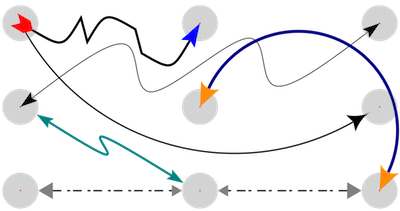
\includegraphics[width=0.47\textwidth]{html/arrows.png}
\end{center}
%*endignore

\subsubsection*{What's new}

Since the last HCAR edition we have seen releases 1.0 and 1.1 and 
the current version 1.2 was released in June 2014.
New features include:
\begin{itemize}
\item An API for drawing arrows including: several ways to connect diagrams
  with arrows, arbitrary shaped shafts, and a collection of arrowheads.
\item Consistent use of the \texttt{lens} package to access and modify 
  record fields and newtypes.
\item Performance improvements of about 30\% obtained by the use
  of better data structures to represent diagram output.
\item Support for 3D diagrams.
\item Introduction of a new measurement type and the removal of the
  freeze function makes things like handling line widths and text sizes
   more flexible.
\item New haskell native backends: \texttt{diagrams-rasterific} and
  \texttt{diagrams-canvas}. 
\item Many other features including support for: linear and radial gradients, tight alignment of convex
  shapes, improved clipping, animated GIFs (in cairo and rasterific), creating offsets paths,
  and both external and embedded images.
\end{itemize}


% %**<img width=400 src="./diagrams-haddock.jpg">
% %*ignore
% \begin{center}
% 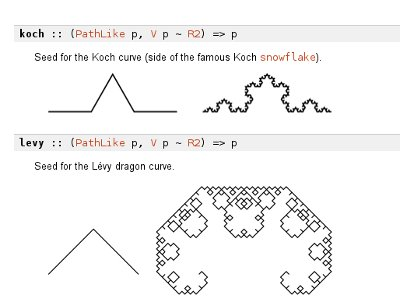
\includegraphics[width=0.4\textwidth]{html/diagrams-haddock.jpg}
% \end{center}
% %*endignore

There have been many improvements and changes to the core
diagrams libraries as well.  The next release of diagrams is
slated to include:
\begin{itemize}
\item Support of handling directions (vectors which have forgotten their magnitude).
  Which will provide a consistent API in all dimensions.
\item Generic scalars values, i.e. not restricted to type 
  Double.
\item A major refactoring of the way vector spaces are handled
  using the \texttt{linear} package.
\item a PGF backend with full TeX support.
\end{itemize}


%**<img width=350 src="./kaleidoscope.png">
%*ignore
\begin{center}
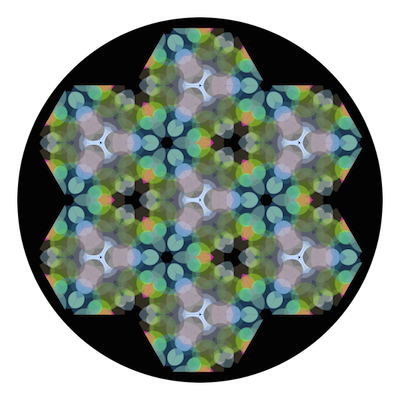
\includegraphics[width=0.45\textwidth]{html/kaleidoscope.png}
\end{center}
%*endignore


%**<img width=350 src="./FibCalls.png">
%*ignore
%\begin{center}
%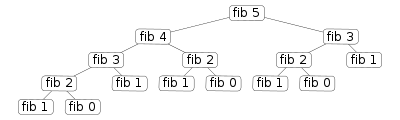
\includegraphics[width=0.33\textwidth]{html/FibCalls.png}
%\end{center}
%*endignore
\subsubsection*{GSoC}

We had two Google Summer of Code projects dedicated to diagrams
projects this past summer.

\begin{itemize}
\item Allan Gardner laid the groundwork for using numeric types beyond
Double.  After several iterations, this led to the adoption of the
\textt{linear} package. This paves the way for using automatic
differentiation, constraint solving, and fixed or dynamic precision
numbers with Diagrams.
\item Niklas Haas  added lenses to diagrams, in order 
to make it possible to (efficiently) traverse over diagrams and 
subdiagrams, modifying them in the process.
\end{itemize}


\subsubsection*{Contributing}

There is plenty of exciting work to be done; new contributors are
welcome!  Diagrams has developed an encouraging, responsive, and fun
developer community, and makes for a great opportunity to learn and
hack on some ``real-world'' Haskell code.  Because of its size,
generality, and enthusiastic embrace of advanced type system features,
diagrams can be intimidating to would-be users and contributors;
however, we are actively working on new documentation and resources to
help combat this.  For more information on ways to contribute and how
to get started, see the Contributing page on the diagrams wiki:
\url{http://haskell.org/haskellwiki/Diagrams/Contributing}, or come
hang out in the \texttt{\#diagrams} IRC channel on freenode.

%**<img width=400 src="./topoform.jpg">
%*ignore
\begin{center}
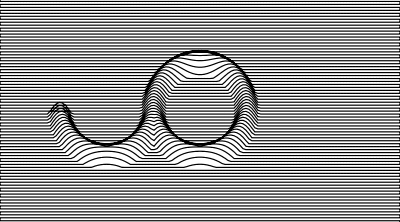
\includegraphics[width=0.4\textwidth]{html/topoform.jpg}
\end{center}
%*endignore

\FurtherReading
\begin{compactitem}
\item \url{http://projects.haskell.org/diagrams}
\item \url{http://projects.haskell.org/diagrams/gallery.html}
\item \url{http://haskell.org/haskellwiki/Diagrams}
\item \url{http://github.com/diagrams}
\item \url{https://byorgey.wordpress.com/2012/08/28/creating-documents-with-embedded-diagrams/}
\item \url{http://www.cis.upenn.edu/~byorgey/pub/monoid-pearl.pdf}
\item \url{http://www.youtube.com/watch?v=X-8NCkD2vOw}
\end{compactitem}
\end{hcarentry}
